\begin{SCfigure*}
	\centering
	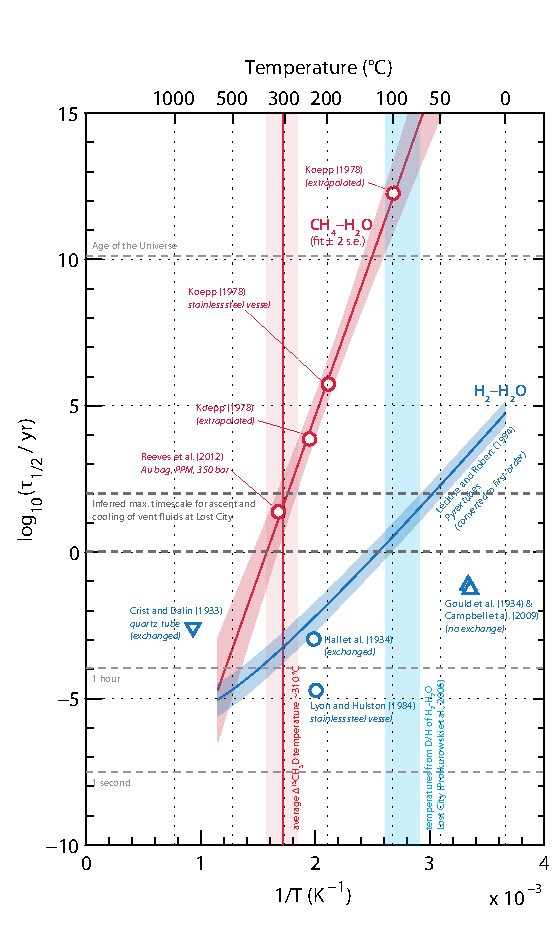
\includegraphics[width=0.625\linewidth]{figures/Fig3.4}
	\caption[Half-exchange timescales for hydrogen exchange between CH\textsubscript{4} \& H\textsubscript{2}O
 and H\textsubscript{2} \& H\textsubscript{2}O ]{%
		Half-exchange time\-scales ($\tau_{1/2} = \ln(2)/k$) for
		hydro\-gen exchange between CH\textsubscript{4} \& H\textsubscript{2}O
		(red sym\-bols) and H\textsubscript{2} \& H\textsubscript{2}O (blue) based
		on experiments done in the absence of added catalyst
		\parencite{Crist+Dalin_1933_JCP,Hall++_1934_JACS,Gould++_1934_JCP,Koepp_1978,Lyon+Hulston_1984_GCA,Lecluse+Robert_1994_GCA,Campbell++_2009_GCA,Reeves++_2012_GCA}.
	 	Reactions were assumed to be first order in
		CH\textsubscript{4} or H\textsubscript{2}. When rate constants were not
		provided by the authors or when exchange was not observed, the reported
		duration of the experiment was taken as an estimate of the timescale of
		exchange. Downward- and upward-pointing triangles are, respectively,
		maximum and minimum estimates of the exchange timescale. The
		$\tau_{1/2}$ for CH\textsubscript{4}--H\textsubscript{2}O
		exchange from \textcite{Reeves++_2012_GCA} comes from \autoref{fig:3:S2}.
		Second-order rate coefficients for
		H\textsubscript{2}--H\textsubscript{2}O exchange from \textcite{Lecluse+Robert_1994_GCA} were converted to first-order rate coefficients by multiplying by
		the equilibrium vapor pressure of H\textsubscript{2}O calculated at
		temperatures \emph{T} and a pressure of 1~kbar. Uncertainties in
		exchange rates are difficult to estimate, but are probably one order of
		magnitude or greater. Clumped isotopologue temperatures for
		CH\textsubscript{4} from the present study (red bar) and temperatures
		from D/H geothermometry of H\textsubscript{2}--H\textsubscript{2}O in
		endmember fluids at the Lost City site (blue bar) \parencite{Proskurowski++_2006_CG} are also shown. See text for interpretation of these data with
		respect to timescales of fluid circulation.
	}
	\label{fig:3:4}
\end{SCfigure*}